\documentclass[12pt]{article}

\usepackage{hyperref} % гиперссылки

\usepackage{tikz} % картинки в tikz
\usepackage{microtype} % свешивание пунктуации

\usepackage{array} % для столбцов фиксированной ширины

\usepackage{indentfirst} % отступ в первом параграфе

\usepackage{sectsty} % для центрирования названий частей
\allsectionsfont{\centering}

\usepackage{amsmath, amssymb, amsthm} % куча стандартных математических плюшек

\usepackage{comment} % добавление длинных комментариев

\usepackage[top=2cm, left=1.2cm, right=1.2cm, bottom=2cm]{geometry} % размер текста на странице

\usepackage{lastpage} % чтобы узнать номер последней страницы

\usepackage{enumitem} % дополнительные плюшки для списков
%  например \begin{enumerate}[resume] позволяет продолжить нумерацию в новом списке

\usepackage{caption} % что-то делает с подписями рисунков :)

\usepackage{qcircuit} % для рисовки квантовых диаграмм
\usepackage{physics} % бракеты

\usepackage{answers} % разделение условий и ответов в упражнениях

\usepackage{chessboard} % рисование шахматной доски


\usepackage{fancyhdr} % весёлые колонтитулы
\pagestyle{fancy}
\lhead{Демоническая оптимизация}
\chead{}
\rhead{КЛШ-2018}
\lfoot{}
\cfoot{}
\rfoot{\thepage/\pageref{LastPage}}
\renewcommand{\headrulewidth}{0.4pt}
\renewcommand{\footrulewidth}{0.4pt}



\usepackage{todonotes} % для вставки в документ заметок о том, что осталось сделать
% \todo{Здесь надо коэффициенты исправить}
% \missingfigure{Здесь будет Последний день Помпеи}
% \listoftodos — печатает все поставленные \todo'шки



\usepackage{booktabs} % красивые таблицы
% заповеди из докупентации:
% 1. Не используйте вертикальные линни
% 2. Не используйте двойные линии
% 3. Единицы измерения - в шапку таблицы
% 4. Не сокращайте .1 вместо 0.1
% 5. Повторяющееся значение повторяйте, а не говорите "то же"



\usepackage{fontspec} % что-то про шрифты?
\usepackage{polyglossia} % русификация xelatex

\setmainlanguage{russian}
\setotherlanguages{english}

% download "Linux Libertine" fonts:
% http://www.linuxlibertine.org/index.php?id=91&L=1
\setmainfont{Linux Libertine O} % or Helvetica, Arial, Cambria
% why do we need \newfontfamily:
% http://tex.stackexchange.com/questions/91507/
\newfontfamily{\cyrillicfonttt}{Linux Libertine O}

\AddEnumerateCounter{\asbuk}{\russian@alph}{щ} % для списков с русскими буквами
\setlist[enumerate, 2]{label=\asbuk*),ref=\asbuk*}

%% эконометрические сокращения
\DeclareMathOperator{\Cov}{Cov}
\DeclareMathOperator{\Corr}{Corr}
\DeclareMathOperator{\Var}{Var}
\DeclareMathOperator{\E}{E}
\def \hb{\hat{\beta}}
\def \hs{\hat{\sigma}}
\def \htheta{\hat{\theta}}
\def \s{\sigma}
\def \hy{\hat{y}}
\def \hY{\hat{Y}}
\def \v1{\vec{1}}
\def \e{\varepsilon}
\def \he{\hat{\e}}
\def \z{z}
\DeclareMathOperator{\hVar}{\widehat{\Var}}
\DeclareMathOperator{\hCorr}{\widehat{\Corr}}
\DeclareMathOperator{\hCov}{\widehat{\Cov}}
\def \cN{\mathcal{N}}

\let\P\relax
\DeclareMathOperator{\P}{\mathbb{P}}



\usepackage[bibencoding = auto,
backend = biber,
sorting = none,
style=alphabetic]{biblatex}

\addbibresource{em1_pset_v2.bib}



% делаем короче интервал в списках
\setlength{\itemsep}{0pt}
\setlength{\parskip}{0pt}
\setlength{\parsep}{0pt}




\Newassociation{sol}{solution}{solution_file}
% sol --- имя окружения внутри задач
% solution --- имя окружения внутри solution_file
% solution_file --- имя файла в который будет идти запись решений
% можно изменить далее по ходу
\Opensolutionfile{solution_file}[all_solutions]
% в квадратных скобках фактическое имя файла

% магия для автоматических гиперссылок задача-решение
\newlist{myenum}{enumerate}{3}
% \newcounter{problem}[chapter] % нумерация задач внутри глав
\newcounter{problem}[section]

\newenvironment{problem}%
{%
\refstepcounter{problem}%
%  hyperlink to solution
     \hypertarget{problem:{\thesection.\theproblem}}{} % нумерация внутри глав
     % \hypertarget{problem:{\theproblem}}{}
     \Writetofile{solution_file}{\protect\hypertarget{soln:\thesection.\theproblem}{}}
     %\Writetofile{solution_file}{\protect\hypertarget{soln:\theproblem}{}}
     \begin{myenum}[label=\bfseries\protect\hyperlink{soln:\thesection.\theproblem}{\thesection.\theproblem},ref=\thesection.\theproblem]
     % \begin{myenum}[label=\bfseries\protect\hyperlink{soln:\theproblem}{\theproblem},ref=\theproblem]
     \item%
    }%
    {%
    \end{myenum}}
% для гиперссылок обратно надо переопределять окружение
% это происходит непосредственно перед подключением файла с решениями


\theoremstyle{definition}
\newtheorem{definition}{Определение}



\begin{document}

\tableofcontents{}

\section*{Цель}

\begin{itemize}
  \item познакомить девятиклассников с основными идеями динамической оптимизации (принцип Беллмана, решение с хвоста, цена позиции, $MR=MC$, пространство состояний);
  \item рассказать классические задачи, составляющие культурный код (разборчивая невеста, определение высоты здания, пираты, \ldots);
\end{itemize}


\newpage
\section{Забери камень}


\begin{problem}

Четыреста лет назад, в 1612 г. в Лионе появилась книга поэта и математика Баше де Мезирьяка
(Claude Gaspar Bachet de M\'eziriac
\footnote{Баше де Мезирьяк перевел с греческого на латынь Арифметику Диофаната,
на полях которой Ферма сформулировал свою великую теорему})
«Занимательные и приятные числовые задачи» (Probl\`emes plaisants et d\'electables qui se font par les nombres).
В ней была предложена следующая игра. Двое по очереди называют числа от 1 до 10, выигрывает тот,
кто первым доведет сумму до 100. В чью пользу эта игра?

Ссылка на переиздание 1884 года \url{http://cnum.cnam.fr/DET/8PY45.html}, задача 22.

\begin{sol}

\end{sol}
\end{problem}



\begin{problem} Цзяньшинцзы «Выбирание камней»

Древний Китай. Две кучки камней. Два игрока ходят по очереди.
За один ход можно забрать либо произвольное число камней из одной кучки,
либо одинаковое число камней из обеих. В одной кучке 5, а в другой — 8 камней.

Кто выигрывает при правильной игре?

\begin{sol}

\end{sol}
\end{problem}


\begin{problem} «Одинокий ферзь»

Шахматная доска, одинокий раненый ферзь стоит на h6.
Раненый ферзь как и ферзь может двигаться на любое число клеток,
но только влево или вниз, или влево-вниз. Двое игроков ходят по очереди,
тот кто переставит ферзя на а1 выиграл.
\begin{enumerate}
\item В чью пользу эта игра? Если в пользу первого, то с какого хода следует начать игру?
\item Какие позиции на доске являются проигрышными и проигрышными, если ферзь очень
сильно ранен и больше чем на два шага пойти не может?
\item Найди 10 отличий игры «Одинокий ферзь» от игры «Цзяньшинцзы».
\end{enumerate}

\def\mylist{Qh6}
\setchessboard{setpieces=\mylist,showmover=false}
\chessboard

\begin{sol}

\end{sol}
\end{problem}

\begin{problem} «Набери чет»

В кучке 135 камней, двое по очереди забирают себе от 1 до 4 камней.
Выигрывает тот, кто к концу игры наберет четное число камней.

Кто выигрывает при правильной игре?

\begin{sol}

\end{sol}
\end{problem}


\begin{problem}

В кучке 147 камней, Полина и Василий по очереди берут камни.
Полина начинает первой. Выигрывает тот, кто возьмёт последний камень.
Полина может взять 1, 4 или 5 камней, а Василий — 1, 3 или 4 камня.

\begin{enumerate}
  \item Кто выигрывает при правильной игре?
  \item Как изменится результат, если Василий может брать 1, 3, 4 или 20 камней?
  \item Как изменится результат, если Василий может брать 1, 3, 4 или 6 камней?
\end{enumerate}

\begin{sol}

\end{sol}
\end{problem}



\begin{problem} Опустошай и разделяй!

Есть две коробочки. В каждой из них лежит некоторое количество камешков.
Игроки ходят по очереди.
За один ход игрок выбрасывает содержимое одной из коробочек,
и затем делит содержимое другой между двумя коробочками.
Как минимум один камешек должен оставаться в каждой коробочке.
Проигрывает тот, кто не может сделать ход по правилам.

Найди все выигрышные позиции.
\begin{sol}

\end{sol}
\end{problem}


\begin{problem} Опустошай и разделяй без равенства!

Есть две коробочки. В каждой из них лежит некоторое количество камешков.
Игроки ходят по очереди.
За один ход игрок выбрасывает содержимое одной из коробочек,
и затем делит содержимое другой между двумя коробочками.
\textbf{Поровну делить нельзя!}
Как минимум один камешек должен оставаться в каждой коробочке.
Проигрывает тот, кто не может сделать ход по правилам.

Каковы есть оптимальные ходы в позиции $7$ и $9$ камешков?
\begin{sol}

\end{sol}
\end{problem}


\newpage
\section{Посади дерево!}

\begin{problem} Рулетки

Есть три рулетки: на первой равновероятно выпадают числа 2, 4 и 9; на второй — 1, 6 и 8;
на третьей — 3, 5 и 7. Сначала первый игрок выбирает рулетку себе,
затем второй игрок выбирает рулетку себе из двух оставшихся.
После этого рулетки, выбранные игроками, запускаются, и случай определяет победителя.
Победителем считается тот, чья рулетка покажет большее число.

Победитель получает от проигравшего 100 рублей.

В чью пользу эта игра?

\begin{sol}
Вероятность выигрыша для второго игрока — $5/9$.
\end{sol}
\end{problem}



\begin{problem} Кортес

Кортес с бандой головорезов высадился на берегу.
Кортес выбирает, нападать ли на деревушку или нет.

Местная деревушка может либо сразу перейти в подчинение Кортеса, либо принять бой.
Если деревушка примет бой, то выбор появится у Кортеса: либо драться до победного конца,
либо после первых потерь бежать на кораблях обратно.

Ценность деревушки для Кортеса — одна единица, ценность собственных головорезов — 2 единицы.
Если Кортес будет драться до конца, то деревушка будет взята,
но большинство головорезов погибнет в бою. Для жителей деревушки — главное остаться в живых,
сохранить при этом независимость, конечно, желательно.

\begin{enumerate}
  \item Нарисуй дерево игры и найди обратно-индукционный исход.
  \item Нарисуй дерево игры и найди обратно-индукционный исход в случае, если Кортес сжёг корабли.
\end{enumerate}

\begin{sol}

\end{sol}
\end{problem}




\begin{problem}
Как будут играть абсолютно рациональные игроки, каждый из которых хочет побольше выиграть?


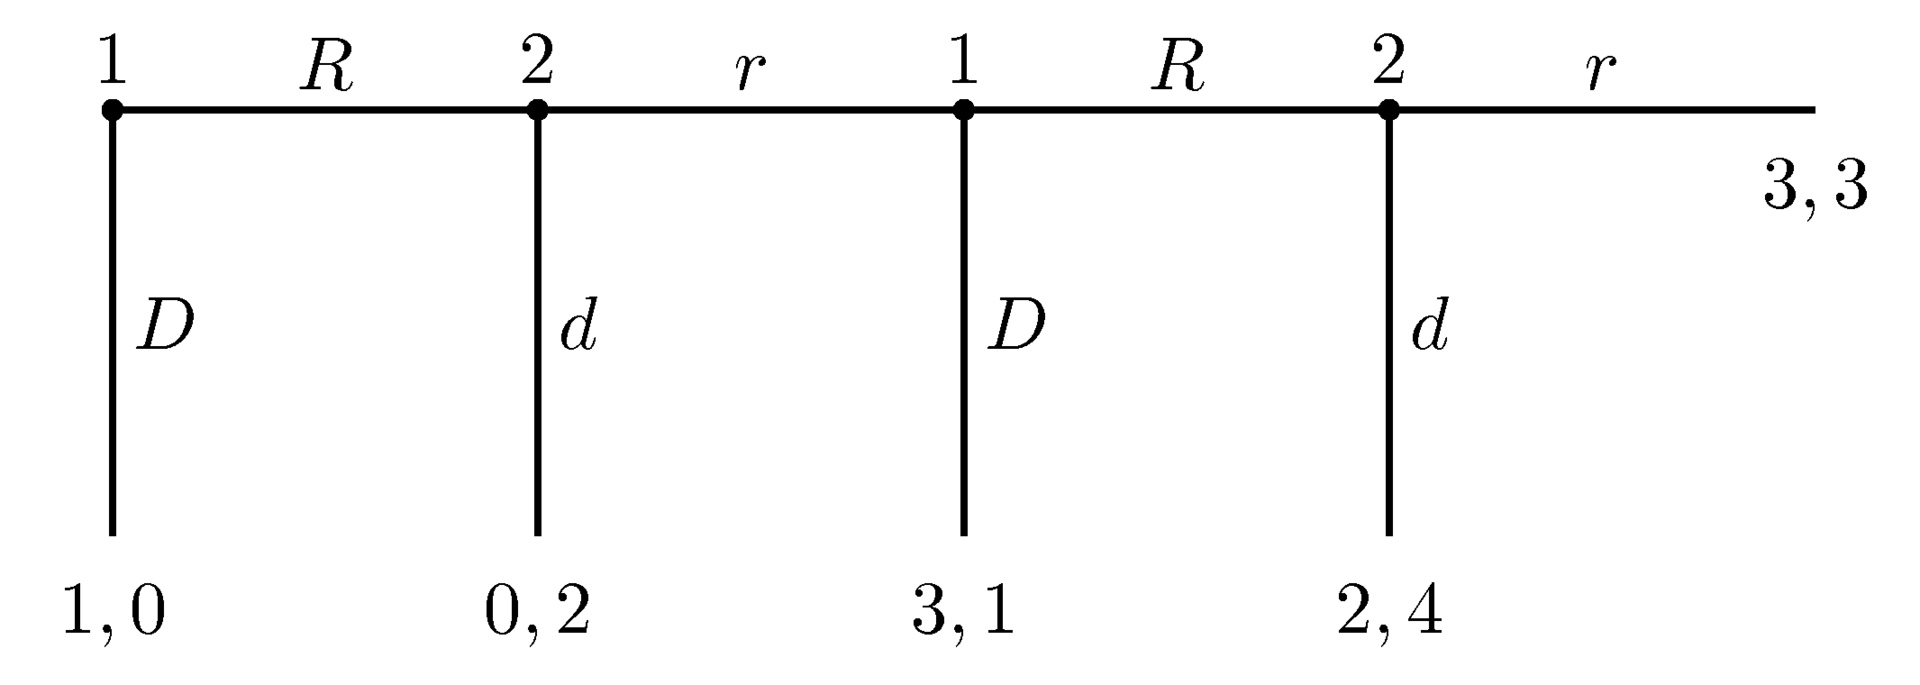
\includegraphics[width=10cm]{images/Centipede_game.png}

\begin{sol}

\end{sol}
\end{problem}



\begin{problem}
Количество денег в волшебной шкатулке каждый день увеличивается!
В день $t$ в шкатулке находится  $1.5\cdot t$  рублей.
Каждый из двух игроков решает, когда ему потребовать деньги.
Тот кто потребует деньги первым — получает сумму полностью, тот,
кто потребует вторым — не получает ничего.
Если требования поступают одновременно, то игроки делят сумму в шкатулке поровну.

На 101-ый день деньги сгорают.


Как будут играть абсолютно рациональные игроки, каждый из которых хочет побольше выиграть?
\begin{sol}

\end{sol}
\end{problem}


\begin{problem}
На острове живут 42 тигра и одна вкусная волшебная антилопа.
 Если тигр съест волшебную антилопу, то он сам превратится в волшебную антилопу.
 Мясо волшебной антилопы настолько вкусно,
 что любой тигр ради его вкуса готов на превращение в антилопу.
 Но ни один тигр не готов полностью расстаться с жизнью ради мяса антилопы.

Тигры охотяться только в одиночку. Другой еды на острове предостаточно.
Что будет происходить на этом острове?
\begin{sol}
  Один тигр съест антилопу, превратиться в неё, а дальше никто антилопу ловить
  не будет.
\end{sol}
\end{problem}

\begin{problem} Мимимишные пираты

На корабле 50 пиратов и они раздобыли 100 золотых слитков. Слитки неделимые.

У пиратов есть строгая иерархия: капитан, первый помощник капитана, второй помощник и т.д.
Пираты делят золото так: сначала капитан предлагает свой вариант дележа,
затем пираты голосуют за или против, если дележ одобрен более чем половиной пиратов,
включая предложившего дележ, то он принимается, если нет, то капитана убивают,
и дележ предлагает первый помощник\ldots

Если пиратов остаётся двое, голосование не проводится и пираты делят золото поровну.

Жизненные ценности мимимишного пирата просты:

\begin{enumerate}
  \item Выжить лучше, чем умереть.
  \item Если в обоих вариантах я жив, то лучше вариант, где у меня больше денег.
  \item Если я жив и одинаково денег, то лучше вариант, где больше \textbf{живых} товарищей.
  \item Если я жив, одинаково денег и живых товарищей, то лучше вариант, где деньги получают старшие.
\end{enumerate}

\begin{enumerate}
  \item Какой делёж будет реализован?
  \item Как изменится ответ для кровожадных пиратов, которые предпочитают \textbf{мёртвых} товарищей?
\end{enumerate}

\begin{sol}
\end{sol}
\end{problem}


\begin{problem}
В стране $1000$ жителей, включая короля, каждый из которых получает заработную плату в одну монету.
Когда в стране победила демократия, король потерял свою власть, даже был лишен права голоса.
Единственное, что он может — так это предлагать перераспределение заработной платы.
Зарплата каждого жителя должна выражаться неотрицательным количеством монет,
в сумме все зарплаты должны равняться $1000$.

Когда король предлагает перераспределение зарплаты, каждый житель,
кроме самого короля, может проголосовать за, против или вообще не приходить на голосование.

Новое распределение одобряется, если число голосов «за» строго больше числа голосов «против».

Каждый житель эгоистичен, голосует «за», если в новом проекте его зарплата растет,
«против», если падает, и не приходит на голосование, если ему предлагается одинаковая зарплата.

Какую зарплату в результате получит хитрый король и сколько голосований ему потребуется?

\begin{sol}
\end{sol}
\end{problem}

\newpage
\section{Состоянье у тебя истерическое}


\begin{problem}
Из города А в город Б ведут две непересекающиеся дороги. Одновременно
из А в Б выехали две машины по этим двум дорогам. Водителям удалось
проехать так, чтобы машины постоянно находились в прямой видимости друг друга.
Финишировали водители в Б одновременно. По дороге водители могли менять скорость.

Теперь водители хотят одновременно стартовать в разных городах, одновременно
финишировать, и проехать, возможно меняя скорость, по двум дорогам так,
чтобы ни разу не оказаться в пределах прямой видимости.

Получится ли у водителей задуманное?
  \begin{sol}
  \end{sol}
\end{problem}


\begin{problem}
Турист прошёл путь из А в Б, стартовав в 9:00 и финишировав в 21:00. Шёл неравномерно,
делая паузы. Проведя в Б несколько дней, турист пошёл обратно, также стартовав в 9:00,
и финишировав в 21:00 в А. И обратно турист шёл неравномерно.

Обязательно ли найдётся такой момент дня, в который турист был в той же самой
точке?
\begin{sol}
\end{sol}
\end{problem}


\begin{problem}
Задача про перестановку коней.
Б Б
Ч Ч
и
Б Ч
Ч Б


\begin{sol}
\end{sol}
\end{problem}




\section{Определение высоты здания}

\begin{problem}
В доме 100 этажей. У тебя два одинаковых хрустальных шара.
Если уронить хрустальные шары с первого этажа, то они не разбиваются,
а если уронить с сотого, то разбиваются.

Ты можешь сбрасывать шары с любого этажа.

Твоя цель — за наименьшее количество бросков гарантированно определить,
начиная с какого этажа разбиваются хрустальные шары.

Сколько бросков при оптимальной стратегии тебе потребуется в худшем случае?

\begin{sol}
\end{sol}
\end{problem}


\begin{problem}
В доме 100 этажей. У пожилого и остроглазого профессора два одинаковых хрустальных шара.
Если уронить хрустальные шары с первого этажа, то они не разбиваются,
а если уронить с сотого, то разбиваются.

Профессор может сбрасывать шары с любого этажа. Трудность в том, что в доме
сломался лифт и профессору приходится ходить по лестнице. Вверх
профессору идти тяжело, а вниз — очень легко.

Профессору нужно при наименьшем пути вверх определить,
начиная с какого этажа разбиваются хрустальные шары.

Сколько этажей вверх при оптимальной стратегии потребуется пройти профессору в худшем случае?

\begin{sol}
\end{sol}
\end{problem}


\newpage
\section{Подбрасывание кубиков и монеток}


\begin{problem}
Джон Сильвер и Билли Бонс по очереди подбрасывают игральный кубик. Кто первым
выбросит шестёрку выигрывает. Джон Сильвер начинает первым.

У кого какие шансы на победу?

\begin{sol}
\end{sol}
\end{problem}


\begin{problem}
Джон Сильвер и Билли Бонс подкидывают монетку. Джон выигрывает если последовательность
ОО выпадет раньше. Билли выигрывает, если РРР выпадет раньше.

\begin{enumerate}
  \item В чью пользу эта игра?
  \item В чью пользу будет игра, если Джон ждёт ООР, а Билли — РОО?
\end{enumerate}

\begin{sol}
\end{sol}
\end{problem}



\begin{problem}
Джон Сильвер подкидывает монетку до тех пор, пока не выпадет ООР.
Чему равен ожидаемый выигрыш Джона в каждом случае:

\begin{enumerate}
  \item За каждый бросок Джон получает один песо от казино.
  \item Джон получает один песо за каждого орла.
  \item Джон получает один песо за каждого орла, следующего за решкой.
\end{enumerate}

\begin{sol}
\end{sol}
\end{problem}

\begin{problem}
Джон Сильвер подкидывает монетку до тех пор, пока не выпадет ООО или РРР.
За каждую решку казино увеличивает возможный выигрыш Джона на один песо.
Если рано или поздно выпадает РРР, то Джон получает свой выигрыш.
Если рано или поздно выпадает ООО, то возможный выигрыш Джона сгорает.

\begin{enumerate}
  \item Чему равна вероятность завершить игру в плюсе, стартуя из каждой точки?
  \item Чему равен ожидаемый выигрыш Джона?
\end{enumerate}
\begin{sol}
\end{sol}
\end{problem}


\begin{problem}
 Вы играете в следующую игру. Кубик подкидывается неограниченное число раз.
 Если на кубике выпадает 1, 2 или 3, то соответствующее количество монет добавляется на кон.
 Если выпадает 4 или 5, то игра оканчивается и Вы получаете сумму, лежащую на кону.
 Если выпадает 6, то игра оканчивается, а Вы не получаете ничего. Изначально на кону лежит ноль рублей.
\begin{enumerate}
\item Какова вероятность того, что игра рано или поздно закончится выпадением 6-ки?
\item Какова ожидаемая продолжительность игры?
\item Чему равен ожидаемый выигрыш в эту игру?
\item Чему равен ожидаемый выигрыш в эту игру, если изначально на кону лежит 100 рублей?
\item Изменим условие: если выпадает 5, то сумма на кону сгорает, а игра продолжается. Как изменятся ответы на предыдущие вопросы?
\end{enumerate}

\begin{sol}
\end{sol}
\end{problem}



\begin{problem}
 В каждой вершине треугольника по ёжику. Каждую минуту с вероятностью $0.5$ каждый ежик
независимо от других двигается по часовой стрелке, с вероятностью
$0.5$ — против часовой стрелки.

Чему равно среднее время до встречи всех ежей в общей вершине?

\begin{sol}
\end{sol}
\end{problem}

\begin{problem}
 Есть три комнаты. В первой из них лежит сыр. Если мышка
попадает в первую комнату, то она находит сыр через одну минуту.
Если мышка попадает во вторую комнату, то она ищет сыр две минуты
и покидает комнату. Если мышка попадает в третью комнату, то она
ищет сыр три минуты и покидает комнату. Покинув комнату, мышка
выходит в коридор и выбирает новую комнату наугад, например, может
зайти в одну и ту же. Сейчас мышка в коридоре. Сколько времени ей
в среднем потребуется, чтобы найти сыр?

\begin{sol}
\end{sol}
\end{problem}

\begin{problem}
Илье Муромцу предстоит дорога к камню. От камня начинаются ещё три дороги.
Каждая из тех дорог снова оканчивается камнем. И от каждого камня начинаются ещё три дороги.
И каждые те три дороги оканчиваются камнем\ldots И так далее до бесконечности.
На каждой дороге живёт трёхголовый Змей Горыныч.
Каждый Змей Горыныч бодрствует независимо от других с вероятностью (хм, Вы не поверите!) одна третья.
У Василисы Премудрой существует Чудо-Карта, на которой видно,
какие Змеи Горынычи бодрствуют, а какие — нет.

Какова вероятность того,
что Василиса Премудрая сможет найти на карте
бесконечный жизненный путь Ильи Муромца проходящий исключительно мимо спящих Змеев Горынычей?

\begin{sol}
\end{sol}
\end{problem}



\section{Когда сказать стоп?}

\begin{problem}
Джон Сильвер подбрасывает монетку до выпадения ООО. За каждую решку
казино увеличивает потенциальный выигрыш Сильвера на один песо.

В любой момент Джон Сильвер может сказать «стоп» и забрать выигрыш. Если ООО
выпадает, то Сильвер не получает ничего.

Как следует играть Сильверу? Чему будет равен его выигрыш при использовании
оптимальной стратегии?

\begin{sol}
\end{sol}
\end{problem}


\begin{problem}
 Вася подкидывает кубик до тех пор, пока на кубике не выпадет единица, или пока он сам не скажет «Стоп». Вася получает столько рублей, сколько выпало на кубике при последнем броске. Вася хочет максимизировать свой ожидаемый выигрыш.
\begin{enumerate}
\item Как выглядит оптимальная стратегия? Чему равен ожидаемый выигрыш при использовании оптимальной стратегии?
\item Какова средняя продолжительность игры при использовании оптимальной стратегии?
\item Как выглядит оптимальная стратегия и чему равен ожидаемый выигрыш, если за каждое
подбрасывание Вася платит 35 копеек?
\end{enumerate}

\begin{sol}
  стоп на 4-5-6 или стоп на 5-6
\end{sol}
\end{problem}



\begin{problem}
 Вам предложена следующая игра. Изначально на кону 0 рублей. Раз за разом подбрасывается правильная монетка. Если она выпадает орлом, то казино добавляет на кон 100 рублей. Если монетка выпадает решкой, то все деньги, лежащие на кону, казино забирает себе, а Вы получаете красную карточку. Игра прекращается либо когда Вы получаете третью красную карточку, либо в любой момент времени до этого по Вашему выбору. Если Вы решили остановить игру до получения трех красных карточек, то Ваш выигрыш равен сумме на кону. При получении третьей красной карточки игра заканчивается и Вы не получаете ничего. Вы заинтересованы в максимальном среднем выигрыше.
\begin{enumerate}
\item Как выглядит оптимальная стратегия, если только что была получена вторая красная карточка? Чему равен средний выигрыш?
\item Как выглядит оптимальная стратегия, если только что была получена первая красная карточка?
\item Как выглядит оптимальная стратегия в исходной игре? Чему равен средний выигрыш?
\end{enumerate}

\begin{sol}
стратегия 1: говорить стоп, если на кону 200 рублей вне зависимости от числа набранных красных карточек

 стратегия 2: если нет красных карточек или одна, то останавливаться при 200 рублях, а при двух карточках останавливаться на 100 рублях.
\end{sol}
\end{problem}







\begin{definition}
Шансы события,
\[
odds(A) = \frac{\P(A)}{1- \P(A)}
\]

Стратегия суммы шансов. Представим себе серию из $n$ независимых испытаний.
Вероятность успеха в $k$-ом испытании равна $p_k$. Наша цель — выбрать последний
успех.

Рассмотрим стратегию $S_k$: пропустить $k-1$ испытания и далее выбрать первое
испытание с успехом. Выберем наилучшую стратегию из стратегий данного типа.

Вероятность успеха при стратегии $S_k$ равна:

\begin{multline}
\P(\text{стратегия } S_k \text{ выигрывает}) = \P(\text{произойдет ровно одно событие из } A_k, A_{k+1}, \ldots, A_n) = \\
= p_k q_{k+1} q_{k+2} q_{k+3} \ldots q_n + q_k p_{k+1} q_{k+2} q_{k+3} + \ldots +
q_k q_{k+1} q_{k+2} \ldots q_{n-1} p_n
\end{multline}

Рассмотрим условие, при котором при $10$ испытаниях $S_8$ хуже $S_9$:

\[
p_8 q_9 q_{10} + q_8 p_9 q_{10} + q_8 q_9 p_{10} \leq p_9 q_{10} + q_9 p_{10}
\]

Переносим два последних слагаемых из левой части в правую и приводим подобные слагаемые:
\[
p_8 q_9 q_{10} \leq p_8 p_9 q_{10} + p_8 q_9 p_{10}
\]

И после деления:

\[
1 \leq \frac{p_9}{1-p_9} + \frac{p_{10}}{1-p_{10}}
\]

Поэтому стратегия суммы шансов формулируется так:

Складываем шансы успехов, начиная с конца,
\[
R_k = \frac{p_n}{q_n} + \frac{p_{n-1}}{q_{n-1}} + \ldots + \frac{p_k}{q_k}
\]

Находим, при каком $k$ впервые сумма $R_k$ превышает $1$. Это и есть оптимальная
стратегия $S_k$.
\end{definition}


\begin{problem}
Вася подкидывает кубик ровно 100 раз. Вася имеет право сказать «Ура» один раз. Если Вася
сказал «Ура» сразу после последнего выпадения шестёрки, то он получает 100 рублей.
Как выглядит оптимальная стратегия?

\begin{sol}
  Согласно теореме о сумме шансов, $0.2 + 0.2 + 0.2 + 0.2 + 0.2 \geq 1$, поэтому
  пропускаем $95$ подбрасываний и выбираем первую шестёрку после этого.
\end{sol}
\end{problem}


\section{Ним-стоимость}

\section{Ним-подобные игры}

\section{Задача о разборчивой невесте}

\begin{problem}
Задача о Разборчивой Невесте, Secretary problem

К Разборчивой невесте выстроилась длинная-длинная вереница из потенциальных женихов.
\footnote{Докторская диссертация член-корреспондента РАН Бориса Березовского
«Разработка теоретических основ алгоритмизации принятия предпроектных решений и их применения»
является обобщением задачи о разборчивой невесте, \url{http://en.wikipedia.org/wiki/Secretary_problem}}
Разборчивая невеста хочет выбрать самого богатого из них и только его!
Потенциальные женихи заходят к Разборчивой невесте по одному в случайном порядке.
Невеста неплохо разбирается в богатстве и всегда может ранжировать всех, с кем она общалась,
по величине богатства. Когда к Разборчивой невесте приходит очередной претендент,
она должна сразу принять решение: выбрать данного кандидата или перейти к следующему.
Вернуться к предыдущим кандидатам невозможно — они обижаются и уезжают.

\begin{enumerate}
\item Как выглядит оптимальная стратегия Разборчивой невесты? Чему равна вероятность выбора самого богатого жениха Разборчивой невестой?
\item Подруга-дурнушка Разборчивой невесты хочет выбрать второго по богатству жениха и только его!
Как выглядит её оптимальная стратегия?
Чему равна вероятность выбора второго по богатству жениха Подругой-дурнушкой?
\end{enumerate}

\begin{sol}

На русском хорошо написана короткая книжка \cite{zade2003nevesta}.
Про подружку согласную на второго красавца изложено в \cite{vanderbei2011postdoc}.


Пусть:

$n$ — количество потенциальных женихов,

$t$ — номер шага, на котором находится невеста,

$G_t$ — вероятность того, что $t$-ый жених лучше всех предыдущих,

$F_t$ — вероятность того, что пропустив $t$ женихов и дальше пользуюясь оптимальной
стратегией (предполагается, что невеста будет пользоваться предложенной стратегией с $t+1$
шага), невеста выберет в мужья самого богатого.

Определим вероятность $G_t$. Очевидно, что $G_n = 1$. Тогда вероятность того, что $n$-ый жених будет лучше всех предыдущих, равна  $\frac{1}{n}$ $\Rightarrow$ $G_{n-1}=1-\frac{1}{n}=\frac{n-1}{n}$ – вероятность "победы" на $n-1$ шаге. Пользуемся дальше подобной логикой. $\frac{1}{n-1}$ – вероятность того, что $n-1$ жених лучше $n-2\Rightarrow$ вероятноть того, что $n-1$ будет не лучше $n-2$ равна $1-\frac{1}{n-1}=\frac{n-2}{n-1}\Rightarrow G_{n-2}= \frac{1}{n-1}\cdot 0+\frac{n-2}{n-1}\cdot G_{n-1}=\frac{n-2}{n}$. Используя метод математической индукции получаем, что $G_t=\frac{t}{n}$.

Теперь найдём $F_t$. Для этого стоит уточнить, что Разборчивая невеста будет пользоваться оптимальной стратегией с $t+1$ шага, то есть всех предыдущих женихов она сразу отвергает. И ещё очень важно заметить, что вероятность успеха невесты в её нелёгком деле не превышает величины $F_t \Rightarrow F_{t+1} \le F_t \Rightarrow F_t$ – убывающая последовательность. Из всего вышесказанного делаем вывод, что $F_n = 0$, так как отвергнув последнего жениха, невеста останется одна $\Rightarrow F_{n-1}=\frac{1}{n}$ - вероятность, что $n$-ый жених лучше всех. Тогда $F_{n-2}=\frac{1}{n-1}\cdot\frac{n-1}{n}+\frac{n-2}{n-1}\cdot\frac{1}{n}=\frac{(n-2)+(n-1)}{n(n-1)}$. В данном случае сразу найти итоговый $F_t$ затрруднительно, поэтому рассмотрим величину $\frac{F_t}{G_t}$, тем более нам всё равно придётся сравнивать дальше эти величины. Получается, что $\frac{F_{n-2}}{G_{n-2}}=\frac{1}{n-1}+\frac{1}{n-2}$ $\Rightarrow$ по методу математической индукции $F_t = \frac{t}{n} \cdot (\frac{1}{t}+\frac{1}{t+1}+\ldots +\frac{1}{n-1})$.

Перейдём к самой стратегии. Представим, что $F_t$ и $G_t$ непрервыные функции(хотя это не так, потому что они зависят от целых чисел). Тогда $F_t$ - монотонно убывающая функция, а $G_t$ монотонно возрастающая и изобразить их в осях $t, P$, где $P$ - вероятность и $E(G_t)=E(F_t)=[0;1]$ ($E$ - область значения), то найдётся такая точка $T$, в которой эти графики пересекутся $\Rightarrow$ надо найти ближайшее целое $t_1$, до которого невеста пропустит всех женихов, а дальше остановится на первом же, который луше всех предыдущих.

Для того, чтобы найти это оптимальное $t_1$, необходимо рассмотреть соотношение $\frac{F_t}{G_t}$ и сравнить его с $1$. Получается, что $\frac{F_t}{G_t}= \frac{1}{t}+\frac{1}{t+1}+\ldots +\frac{1}{n-1}$, для $t \ge t_1$.

Предположим, что $n, t$ - достаточно большие числа, которые позволят нам перейти к рассматриванию функций. Заметим, что если нарисовать график $y=\frac{1}{x}$, отметить точки $t, t+1,\ldots , n$ и нарисовать прямоугольники с длиной соответствующей  $\frac{1}{t}, \frac{1}{t+1},\ldots ,\frac{1}{n}$ и шириной $1$, то сумма площадей этих прямогольников будет соответствовать $S = \frac{1}{t}+\frac{1}{t+1}+\ldots +\frac{1}{n-1}$.

Если произвети сжатие и растяжение функции $y=\frac{1}{x}$ в t раз, величина $\frac{1}{t}$ станет очень маленькой $\Rightarrow$ сумма площадей прямоугольников практически в точности будет соответствовать площади под графиком на отрезке $[t, n]$. Заметим, что равенство $S(xy)=S(x)+S(y)$ выполняется для всех $x, y>1$, что соответсвует одмому из свойств логарифмов $\Rightarrow S(x)=log_a(x)\Rightarrow$ для обратой функциии будет выполняться $H(x+y)=H(x)*H(y)\Rightarrow$ это показательная функция $H(x)= a^x$. В итоге получаем, что $a$ – это то самое число, которое нам надо узнать для того, чтобы найти $S(x)$. Так как $H(1)=a \Rightarrow F(a)=1 \Rightarrow$ рассмотрим различные значение пложади под $y=\frac{1}{x}$. $S(2)<1\Rightarrow a>2, S(2,5)<1 \Rightarrow a>2,5 , S(3)>1 \Rightarrow a<3 \Rightarrow$ интуитивно понятно, что $a = e$.
В итоге имеем, что $\frac{F_t}{G_t}=1 \Leftrightarrow \frac{n}{t}=e \Leftrightarrow \frac{t}{n}=\frac{1}{e}\Rightarrow F_t=G_t=\frac{t}{n}=\frac{1}{e}\Rightarrow$ вероятность «успеха» невесты найти самого богатого $\frac{1}{e}\approx 0,368$.

А оптимальная стратегия такова: пропустить $\approx 36,8\%$ женихов и выбрать первого же, который будет лучше всех своих предшественников.
\end{sol}

\end{problem}

\section{Труэль}


\begin{problem}
Труэль

Три игрока решили стреляться ради самой красивой девушки и организуют труэль (дуэль для трёх игроков).  Игроки стреляют по очереди, $A$-$B$-$C$-$A$-\ldots. Каждый из игроков может либо целиться в одного из противников, либо стрелять в воздух. Вероятности попадания равны $p_a=0.6$, $p_b=0.5$ и $p_c=0.4$, соответственно. Игра продолжается до определения единственного победителя, он и получает девушку в жёны.

\begin{enumerate}
\item Как выглядит оптимальная стратегия каждого игрока?
\item Чему равные вероятности выиграть для каждого игрока?
\end{enumerate}

\begin{sol}
\textbf{Оптимальные стратегии}

Оптимальная стратегия игрока А (вероятность попадания 0.6) - в любом случае будет стрелять в противника, так как его вероятность попасть больше, чем у остальных, а вероятность, что попадут в него, меньше.

Оптимальная стратегия игрока С (вероятность попадания 0.4) - стрелять в воздух до того момента, как в игре останутся два игрока (С + А/В). Так он дает сильным игрокам возможность "разобраться" друг с другом, и если один убивает другого, то следующим ходом он первым имеет возможность уничтожить оставшегося ( пусть и с небольшой вероятностью). В противном случае, если он убивает А, то следующим ходом с большой вероятность В убьет его самого.

Оптимальная стратегия игрока В (вероятность попадания 0.5) совпадает со стратегией игрока А (может быть, В и выгодно бы было отклонятся, но он понимает стратегию С и в таком случае не будет стрелять в воздух).

\textbf{Решение по дереву вероятностей}

\begin{figure*}
    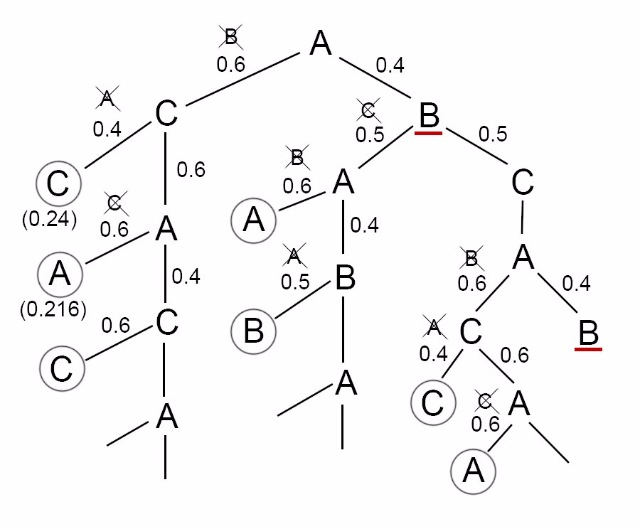
\includegraphics[width=10cm]{images/truel_task37.jpg}
\end{figure*}
\begin{enumerate}
\item Если первым выстрелом А убил В (с вероятностью 0.6), то шанс победить остается у А и у С. Вероятность, что дальше С попадет в цель своим первым выстрелом и победит = 0.24. Если же С промахивается, а следующим ходом А его убивает, то А побеждает с вероятностью 0.216. Если А промахивается, то исход дуэли решает С и цикл повторяется. Можно заметить, что вероятность победы любого из них - сумма бесконечно убывающей геометрической прогресии.

$\P(\text{победа C})= \frac{0.24}{1-0.24} = 0.32$

$\P(\text{победа A}) = \frac{0.216}{1-0.24} = 0.28$
\item Если первым выстрелом А не убивает В, то

а) следующим ходом В убивает С и победа разыгрывается между А и В;

б) В не убивает С, тогда (С стреляет в воздух) либо А убивает В, либо промахивается, и ход опять падает на В (при этом все живы) - цикл повторяется.

а) $\P(\text{победа A}) = \frac{0.12}{1-0.2} = 0.15$

$\P(\text{победа B}) = \frac{0.04}{1-0.2} = 0.05$

б) Теперь можно учесть повтор цикла для вероятности А и В (случай, когда А промахнулся и ход опять перешел В)

$\P(\text{победа A}) = \frac{0.15}{1-0.2} = 0.19$

$\P(\text{победа B}) = \frac{0.05}{1-0.2} = 0.06$

Если же А сразу убивает В, то (учитывая все циклы)

$\P(\text{победа A}) = \frac{\frac{0.0432}{1-0.24}}{1-0.2} = 0.07$

$\P(\text{победа C}) = \frac{\frac{0.048}{1-0.24}}{1-0.2} = 0.08$

\textbf{Проверим сумму вероятностей}: $0.32 + 0.28 + 0.19 + 0.06 + 0.07 + 0.08 = 1 $

\textbf{Результат}:

$\P(\text{победит A}) = 0.28 + 0.19 +0.07 = 0.54$

$\P(\text{победит B}) = 0.06$

$\P(\text{победит С}) = 0.32 + 0.08 = 0.4$
\end{enumerate}
\end{sol}

\end{problem}


\section{Задача о делении ставки}

\begin{problem}
У домашнего учителя Алексея Ивановича один фридрихсдор.
Перед ним обычная колода в 52 карты.
Перед открытием каждой карты Алексей Иванович выбирает,
какую долю своего богатства, от нуля до единицы, поставить на цвет следующей карты.
Карты бывают двух цветов: чёрные и красные. Например, у Алексея Ивановича есть такая стратегия:
не ставить ничего вплоть до последней карты и затем поставить весь рубль на нужный цвет.
Такая стратегия гарантированно удвоит его богатство.

Найдите стратегию, которая максимизирует гарантированный выигрыш Алексея Ивановича.
Чему равен этот максимальный гарантированный выигрыш?
\begin{sol}

\end{sol}

\end{problem}



\section{Сходитесь!}

\begin{problem}
Примирение невозможно, и потому Андрей и Борис решаются на дуэль.

\begin{sol}

\end{sol}

\end{problem}



\begin{problem}
Истеричная певица

Начинающая певица дает концерты каждый день. Каждый ее концерт приносит продюсеру 0.75 тысяч евро. После каждого концерта певица может впасть в депрессию с вероятностью 0.5. Самостоятельно выйти из депрессии певица не может. В депрессии она не в состоянии проводить концерты. Помочь ей могут только цветы от продюсера. Если подарить цветы на сумму $0\le x\le 1$ тысяч евро, то она выйдет из депрессии с вероятностью $\sqrt{x}$.

Какова оптимальная стратегия продюсера? Продюсер максимизирует текущую ожидаемую ценность певицы.

\begin{sol}
  Рассмотрим совершенно конкурентный невольничий рынок начинающих певиц. Певицы в хорошем настроении продаются по $V_1$, в депрессии — по $V_2$. Получаем систему уравнений:
\[
\begin{cases}
  V_1 = 0.75 + (0.5 V_1 + 0.5 V_2) \\
  V_2 = \max_x \sqrt{x}V_1 + (1 - \sqrt{x})V_2 - x
\end{cases}
\]
Оптимизируем и получаем, $x^* = (V_1 - V_2)^2/4$. Из первого уравнения находим $(V_1 - V_2)/2=0.75$.
\end{sol}

\end{problem}




\section{Биномиальная модель цены акции}

\section{Опционы американского типа}


\section{Идеи}

\begin{enumerate}
  \item Начинай с хвоста
  \item Сделай первый шаг
  \item Цена позиции
  \item условие безразличия для пороговых стратегий
  \item нарисуй на плоскости
\end{enumerate}


\section{Лог}

\begin{enumerate}
  \item Было 8 школьников, 9-10 класс. Решили 1.1. Сформулировали принципы.
  За $+$ обязательно найдётся $-$, за $-$ идут только плюсы.
  Рассчитываем на 1 шаг вперёд, и далее пользуемся уже рассчитанным.
  Начинай с хвоста. Предположение о рациональности игроков.  Затем 1.3, 1.4. и 1.5.
  \item Задача 2.1. Для сравнения рулеток сформулировали идею «нарисуй на плоскости».
  Задача 2.2. Сформулировали «все игроки знают правила игры». И варианты
  ходов, и платежи, известны обоим игрокам. Далее 2.3 — 2.5.
  В задаче 2.3 изображаем ходы двух игроков в матрице, то есть это
  «нарисуй на плоскости». Про тигров задача очень понравилась. На доске написал
  таблицу жизненных ценностей тигра.
  \item Решили задача 2.6 — 2.7. Одна школьница болела.
  \item На примере простой лотерии выяснили, как считается математическое
  ожидание. На примере задачи 5.1 про Джона Сильвера: выяснили, что вероятности на
  траектории умножаются. Решая задачу про Джона Сильвера с конца нашли вероятность
  вероятность победы каждого игрока. Проговорили снова принципы решения.
  Решили задачу про Джона Сильвера складывая прогрессии. Далее я попытался
  рассмотреть модификацию задачи про Джона Сильвера, мы её не дорешали,
  а она оказалась при прорешивании пост-фактум довольно громоздкой.
  \item Решили 5.2, 5.3, нарисовали картинку для 5.4.
  \item Решили 5.4, 5.5 пункты 1 и 2. Система из четырёх линейных уравнений с
  ожиданием ООО и РРР в 5.4. довольно громоздка для школьников, разумно ждать ОО и РР.
  \item Обсуждая неспешно решили 5.5 (3, 4, 5) и 5.6.
  \item Сначала предложил школьникам вопрос: самый холодный воздух за час до рассвета,
  в момент, когда появляется солнце, через час после рассвета. Идея: наименьшая
  температура в момент, когда скорость остывания сравняется со скоростью нагрева воздуха.
  Затем решили 6.1 и 6.2 (1). Лучше было их решать в обратном порядке.
\end{enumerate}



\Closesolutionfile{solution_file}

% для гиперссылок на условия
% http://tex.stackexchange.com/questions/45415
\renewenvironment{solution}[1]{%
         % add some glue
         \vskip .5cm plus 2cm minus 0.1cm%
         {\bfseries \hyperlink{problem:#1}{#1.}}%
}%
{%
}%

\section{Решения}
\protect \hypertarget {soln:1.1}{}
\begin{solution}{{1.1}}
  $\P(X=1)=3/5$, $\P(X=2)=3/10$, $\P(X=3)=1/10$, $\E(X)=1.5$
\end{solution}
\protect \hypertarget {soln:1.2}{}
\begin{solution}{{1.2}}
\end{solution}
\protect \hypertarget {soln:1.3}{}
\begin{solution}{{1.3}}
\end{solution}
\protect \hypertarget {soln:1.4}{}
\begin{solution}{{1.4}}
   N 3 4 5

  2/8 3/8 3/8
\end{solution}
\protect \hypertarget {soln:2.1}{}
\protect \hypertarget {soln:2.2}{}
\protect \hypertarget {soln:2.3}{}
\protect \hypertarget {soln:2.4}{}
\protect \hypertarget {soln:3.1}{}
\begin{solution}{{3.1}}
\end{solution}
\protect \hypertarget {soln:3.2}{}
\begin{solution}{{3.2}}
\end{solution}
\protect \hypertarget {soln:10.1}{}
\begin{solution}{{10.1}}
  
\end{solution}
\protect \hypertarget {soln:11.1}{}
\begin{solution}{{11.1}}
  
\end{solution}
\protect \hypertarget {soln:11.2}{}
\begin{solution}{{11.2}}
  Например, $CNOT = \ketbra{00}{00} + \ketbra{01}{01} + \ketbra{10}{11} + \ketbra{11}{10}$.
\end{solution}


\section{Источники мудрости}
\printbibliography[heading=none]


\end{document}
